\documentclass[a4paper,12pt]{article}
\usepackage{latexsym}
\usepackage{array}
\usepackage{amsmath}
\usepackage{amsfonts}
\usepackage{bm}
\usepackage{color}
\usepackage{colortbl}
\usepackage{cite}
\usepackage{float}
\usepackage{graphicx}
\usepackage{ulem}
\usepackage{booktabs}
\usepackage[Symbol]{upgreek}
\usepackage{subfigure}
\usepackage{stfloats}
\usepackage{threeparttable}
\usepackage{theorem}
\usepackage{times}
\usepackage{dcolumn}
\usepackage{multirow}
\usepackage[boxed]{algorithm2e}
\usepackage{framed}

\newtheorem{theorem}{\bf Theorem}
\newtheorem{proposition}{\bf Proposition}
\newtheorem{lemma}{\bf Lemma}
\newtheorem{definition}{Definition}
\newtheorem{remark}{\bf Remark}


\setlength{\textheight}{245mm}
\setlength{\textwidth}{170mm}
\setlength{\topmargin}{-15mm}
\setlength{\oddsidemargin}{-5mm}
\setlength{\evensidemargin}{-5mm}
\flushbottom
\setlength{\parindent}{0pt}
\setlength{\baselineskip}{17pt}
\setlength{\parskip}{3mm}
\setlength{\columnsep}{8mm}
\renewcommand{\baselinestretch}{1.65}
\hyphenation{op-tical net-works semi-conduc-tor IEEEtran}
\DeclareGraphicsRule{.png}{eps}{.bb}{}

\newcommand{\PreserveBackslash}[1]{\let\temp=\\#1\let\\=\temp}
\newcommand{\red}[1]{\textcolor{red}{#1}}
\newcommand{\blue}[1]{\textcolor{blue}{#1}}

\newenvironment{IEEEproof}{{\it Proof. }}{}
\newcolumntype{C}[1]{>{\PreserveBackslash\centering}p{#1}}
\newcolumntype{R}[1]{>{\PreserveBackslash\raggedleft}p{#1}}
\newcolumntype{L}[1]{>{\PreserveBackslash\raggedright}p{#1}}

\def \T {^{\mathsf{T}}}
\def \H {^{\mathsf{H}}}
\def \ri {{\rm i}}
\def \d {{\rm d}}

\def\onecol{}

\begin{document}

\begin{center}
 {\Large\bf Sensing RISs: Enabling Dimension-Independent CSI Acquisition for Beamforming}
\end{center}
\begin{center}
 {\Large\bf (Original paper ID: IT-22-0267)}
\end{center}
\begin{center}
 {\Large\bf Response Letter}
\end{center}
\begin{center}
Jieao Zhu, {\it Student Member,~IEEE}, Kunzan Liu, {\it Student Member,~IEEE}, \\ Zhongzhichao Wan, {\it Student Member,~IEEE}, Linglong Dai, {\it Fellow,~IEEE}, \\  Tie Jun Cui, {\it Fellow,~IEEE}, and H. Vincent Poor, {\it Life Fellow,~IEEE} 

\end{center}
\vspace*{+2mm}
\begin{center}
 {\Large\bf Response to Editor's Comments}
\end{center}


\textbf{Editor}: Manuscript ID IT-22-0267 titled ``Sensing RISs: Enabling Dimension-Independent CSI Acquisition for Beamforming'' which you submitted to the IEEE Transactions on Information Theory, has been reviewed.  The comments of the reviewer(s) are included at the bottom of this letter. There may be additional comments as separate files available through your Author Center on the ScholarOne Manuscripts web site, so please check there also to make sure you have received all reviewer comments.

Based on my own detailed reading of the paper and the reviewers' comments, I recommend that you revise and resubmit your manuscript. Specifically, in your revision, the following points must be addressed:

1) Two out of the three reviewers have pointed that the paper is missing a strong information-theoretic element. I would recommend to consider adding results that address that concern.

2) Another major concern is that methods appear ad-hoc and not particularly novel. Again, it is important to address this concern directly.

One of the reviewers has expressed support for the paper, so I hope you will take a step back and consider revisiting the paper to address all the concerns in a significant manner.

\begin{center}
    {\Large\bf Response to Reviewer 1's Comments}
\end{center}

{\textbf{Reviewer 1:}}
This work presents a very interesting idea of enabling CSI acquisition at the RIS without dimension dependent amount of pilots. There's no such work in literature right now so this idea is likely to get a lot of attentions for citations. However, I have the following concerns for the authors to consider. 

{\color{blue}{\textbf{Authors: } 
We appreciate the reviewer's concise summary of the key points of this paper and the positive evaluations on our work. We have tried our best to revise the paper according to the reviewer's valuable comments, and our responses are provided in a point-to-point manner as follows. 
}}

\textbf{Reviewer 1:}
1) Compared to the conventional RIS channel estimation performed at the receiver, this proposed scheme has the following limitations: 1.1) assuming BS-RIS link is known; 1.2) assuming direct BS-user link is blocked; 1.3) the number of sensors is dimension-dependent in exchange of saving pilot. It would be helpful if the authors can list these disadvantages and discuss how to mitigate them if the assumptions cannot be met. For example, would learning help in reducing sensors?

{\color{blue}{\textbf{Authors: } 
Much thanks for pointing out these three limitations of our proposed sensing RIS-based channel estimation scheme. Our efforts to mitigate these disadvantages are listed as follows: 

1.1) The assumption of a known BS-RIS link. There are three possible ways to mitigate the requirement of this prior knowledge. 
First, we can exploit the geometry associated with the BS and RIS. Usually, the location, orientation, aperture size and antenna spacing are fixed after the installation of the BS and RIS, and the BS-RIS link is often free of unpredictable obstructions. 
As a result, the channel phase-shifts between the BS and RIS, i.e., the phases of the channel $\bm G$ in our paper \red{fix here}, are uniquely determined by the above geometric parameters and the operating wavelength. 
Second, even if it is sometimes difficult to obtain the geometric data, we can estimate the channel $\bm G$ with a much longer period thanks to the quasi-static, i.e., slow-varying  property of the BS-RIS link [R1]. This quasi-static property is due to the immobile nature of the BS and the RIS. 
Thus, we can mitigate the additional channel estimation overhead for the BS-RIS channel in a long-term time-averaged sense.

1.2) The assumption that the direct BS-user link is blocked. Thanks again for pointing out this problem, and we have conceived a possible solution to integrate the direct BS-RIS link ${\bm h}_{\rm d}\in\mathbb{C}^{M\times 1}$ into our proposed scheme. Since the direct link does not affect the creation of the IRF, the RIS phase-shift matrix $\bm \Theta$ can be obtained as if there were no such direct link, up to an undetermined global phase $e^{\ri \phi}$. Note that this IRF-based procedure consumes 3 time slots. After this procedure, two uplink training symbol can be transmitted at the user. The uplink channel model is 
\begin{equation}
    \begin{aligned}
        {\bm y}_{\rm BS} &= ({\bm h}_{\rm d} + e^{\ri \phi}{\bm G}\T {\bm \Theta} {\bm f}^*) s' + {\bm n} \\
        &= ({\bm h}_{\rm d} + e^{\ri \phi}{\bm h}_{\rm RIS})s' + {\bm n}.
    \end{aligned}  
\end{equation}
In the first symbol period $\phi$ is set to 0, and in the second $\phi=\pi$. Thus, the direct BS-user link ${\bm h}_{\rm d}$ and the reflective link ${\bm h}_{\rm RIS}$ can be recovered by 
\begin{equation}
    \begin{aligned}
        \hat{\bm h}_{\rm d} &= \frac{{\bm y}_{{\rm BS}, 1} + {\bm y}_{{\rm BS}, 2}}{2},\\
        \hat{\bm h}_{\rm RIS} &= \frac{{\bm y}_{{\rm BS}, 1} - {\bm y}_{{\rm BS}, 2}}{2}. 
    \end{aligned}
\end{equation}
After obtaining the estimators of these two links, the global phase $\phi$ should be tuned to maximize the total channel energy $\| {\bm h}_{\rm d} + e^{\ri \phi}{\bm h}_{\rm RIS} \|^2$, and this is done by setting 
\begin{equation}
    \hat{\phi} = \arg(\hat{\bm h}_{\rm RIS}\H \hat{\bm h}_{\rm d}).
\end{equation}
Though the final solution $\exp(\ri \hat{\phi}) {\bm \Theta}$ for the RIS phase-shift matrix is suboptimal in general, it only consumes two additional 2 slots, resulting in 5 time slots in total for configuring $N$ reflective elements of the RIS. This pilot overhead is still dimension-independent. 

1.3) The assumption that the number of sensors is dimension-dependent in exchange of saving pilots. In general, it is impossible to correctly configure all the $N$ reflective RIS elements if we only have a dimension-independent number of observations available and without any other knowledge about the channel. However, if we assume the channel is sparse in the virtual domain [R2], then the number of observations needed, i.e., the number of sensors in the proposed scheme, can be significantly reduced, while the benefit of dimension-independent pilot overhead is preserved. Without loss of generality, let us consider a RIS-aided SISO scheme with the BS-RIS channel denoted by ${\bm g}\in\mathbb{C}^{N\times 1}$, and the RIS-user link is ${\bm h}\in\mathbb{C}^{N\times 1}$. Further assume that both of the channels are sparse in the angular domain, i.e., ${\bm g} = {\bm A}\tilde{\bm g}$ and ${\bm h} = {\bm A}\tilde{\bm h}$ for some sparse dictionary matrix ${\bm A}$, where $\tilde{\bm g}$ and $\tilde{\bm h}$ are sparse. Then, the power observation ${\bm p}\in\mathbb{R}_{+}^N$ can be represented as 
\begin{equation}
    {\bm p}(\delta) = \left|{\rm blkdiag}(e^{\ri \delta}{\bm A}, {\bm A}) \begin{bmatrix} \tilde{\bm g} \\ \tilde{\bm h}\end{bmatrix} \right|_2^2,
\end{equation}
where $\delta$ is a tunable global phase at the BS transmitter. Thus, by changing $\delta$ within some predefined index set $\Delta$, one can obtain a series of different power observations $\{{\bm p}(\delta)\}_{\delta\in\Delta}$, which corresponds to different IRF patterns. 
Thus, the goal is to retrieve the complex sparse vectors $\tilde{\bm g}$ and $\tilde{\bm h}$ from the phaseless observations $\{{\bm p}(\delta)\}_{\delta\in\Delta}$. 

Fortunately, this problem is usually termed {\it sparse phase retrieval}, and is well-addressed in [R3]. The standard problem formulation for dictionary matrix ${\bm A}\in\mathbb{C}^{M\times N}$ and compressed observations ${\bm y}\in\mathbb{R}_{+}^{M}$ ($M\ll N$) is given by  
\begin{equation}
    \begin{aligned}
        &{\text{find sparse}}~~{\bm x\in\mathbb{C}^N},\\
        &{\text{s.t.}}~~~~~~~~~~~~~~{\bm y} = \left|{\bm A}{\bm x}\right|.
    \end{aligned}
\end{equation}
Since it is possible to retrieve the $K$-sparse ${\bm x}$ with $M\geq 4K-2$ power measurements [R3], we can significantly reduce the number of power sensors on sensing RIS from $N$ to approximately $4K-2$, where $K$ is the sparsity of the concatenated vector ${\bm x} = [\tilde{\bm g}\T, \tilde{\bm f}\T]\T$. In conclusion, with the sparse assumption on the channel, it is possible to significantly reduce the number of required sensors from a dimension-dependent value $N$ to a sparsity-dependent value $4K-2$. 

[R1] C. Hu, L. Dai, S. Han, and X. Wang, ``Two-timescale channel estimation for  reconfigurable intelligent  surface  aided  wireless  communications,'' {\it IEEE Trans. Commun.}, vol. 69, no. 11, pp. 7736-7747, Nov. 2021.

[R2] V. V. Veeravalli, Y. Liang, and A. M. Sayeed, ``Correlated MIMO wireless channels: capacity, optimal signaling, and asymptotics,'' {\it IEEE Trans. Inf. Theory}, vol. 51, no. 6, pp. 2058-2072, Jun. 2005. 

[R3] P. Schniter, and S. Rangan, ``Compressive phase retrieval via generalized approximate message passing,'' {\it IEEE Trans. Signal Process.}, vol. 63, no. 4, pp. 1043-1055, Apr. 2014. 

}}

\textbf{Reviewer 1:}
2) One advantage that's lack mentioning is that the proposed scheme require less number of time slots for channel estimation, which should be used to normalize the SNR for performance comparison.

{\color{blue}{\textbf{Authors: } 
Thanks for the reviewer's insightful suggestions. In order to ensure fair comparison between different channel estimation schemes, we have conducted new simulations and tested all these schemes with a unified assumption. To be specific, we assume a block-fading Rayleigh channel with $B$ symbols for each block, i.e., the random channel matrices $\bm G$ and $\bm f$ are generated once for every consecutive $B$ symbols. Within these $B$ symbols, there are $N_p$ pilot symbols (the number of time slots for pilot signals) for channel estimation, and $N_d$ data symbols for data transmission. The pilot symbols have a total energy of $E_p$, and the data symbols have a total energy of $E_d$.
To ensure that the average transmit power of each block is $P$, the energy values $E_p$ and $E_d$ satisfy 
\begin{equation}
    P=\frac{E_p+E_d}{B}.
\end{equation}
Thus, if the number of pilot symbols $N_p$ are smaller for some scheme, then the average pilot signal-to-noise ratio (SNR) $\gamma_p = E_p/(N_p \sigma_n^2)$ would be automatically higher, ensuring fair comparison in the sense that equal energy is injected into the signal for different channel estimation schemes.   

According to the reviewer's advice, we have improved our simulations by replacing the overall transmit SNR $\gamma = P_{\rm BS}/\sigma_n^2$ by the normalized pilot SNR $\gamma_p=E_p/(N_p \sigma_n^2)$ and the normalized data SNR $\gamma_d=E_d/(N_d\sigma_n^2)$ ($B=N_p+N_d$). 
Since our proposed scheme requires simultaneous signaling from both the BS and the user, the actual transmit power is determined by 
\begin{equation}
    \begin{aligned}
        P_{{\rm BS}, p} &= \frac{E_p}{N_p}P_{\rm max},\quad P_{{\rm BS}, d} = \frac{E_d}{N_d}P_{\rm max}, \\
        P_{{\rm u}, p} &= \frac{E_p}{N_p}P'_{\rm max},\quad P_{{\rm u}, d} = \frac{E_d}{N_d}P'_{\rm max},
    \end{aligned}
    \label{eqn:transmit_power}
\end{equation}
which incorporates the overall BS transmit power budget $P_{\rm max}$, the user transmit power budget $P'_{\rm max}$, and the power allocation between pilot symbols and data symbols.  
The simulation parameters are summarized in the following {\bf Table~\ref{tab:pilot overhead comp CE}}:
\begin{table}[h]
    \color{blue}
    \centering
    \begin{threeparttable}
        \caption{Fair Pilot Overhead Comparison of Different CSI Acquisition Methods} 
        \label{tab:pilot overhead comp CE}
        \begin{tabular}{l|c|c|c|c|c}
            \toprule
            CSI acquisition method  & $N_p$     & $N_d$ & $B$                   & $E_p$                 &  $E_d$            \\ 
            \hline 
            LMMSE $\bm H$           & 200       & 800   & \multirow{3}*{1000}   & \multirow{3}*{50}     & \multirow{3}*{950}\\
            \cline{1-3}
            LMMSE $\bm f$           & 25        & 975   & ~                     & ~                     & ~                 \\
            \cline{1-3}
            Proposed IRF            & 3         & 997   & ~                     & ~                     & ~                 \\ 
            \bottomrule
        \end{tabular}
    \end{threeparttable}
\end{table}

Thus, the fairness between different CSI acquisition schemes is guaranteed by SNR values normalized with the number of pilot time slots. Note that in the above {\bf Table~\ref{tab:pilot overhead comp CE}}, the RIS size $N_z\times N_y$ is set to be $20\times 10$, and the number of BS antennas is set to be $M=8$. As a result, $N_p = 200$ pilots are needed for estimating the cascaded channel $\bm H$, and $N_p = 200/8=25$ pilots are needed for estimating the RIS-user link $\bm f$. Detailed explanation about the LMMSE $\bm H$ and LMMSE $\bm f$ schemes are provided in our response to the next question. 

}}

%% 
\textbf{Reviewer 1:}
It is understood that the conventional channel estimation technique of Sec.II.B requires $P$ time slots. How is $P$ determined? If $P$ equals to the time slots/pilot cost of the proposed scheme, how would the performance comparison be?

{\color{blue}{\textbf{Authors: } 
Thanks to the reviewer for pointing out the vague explanation about the number of required pilot slots $P$ in Sec.II.B. 
We have changed the notation $P$ to $N_p$, i.e., number of pilots, for clarity, and re-do all the related simulations. 
In the first version of this paper, we have compared our proposed IRF-based scheme with the LS channel estimation scheme. However, the LS scheme is able to output the complete cascaded channel $\bm H$ without any prior knowledge, while our proposed IRF-based scheme needs the prior knowledge of the BS-RIS channel $\bm G$. This leads to unfair comparison, since the prior knowledge of different schemes have to be the same. To ensure fair comparison, we have introduced another baseline called the LMMSE-$\bm f$ scheme, by assuming known $\bm G$ and applying LMMSE estimator for the unknown RIS-user link $\bm f$. 

The baselines are compared with our proposed scheme in {\bf Table 2}. For the LS estimators (equivalent to the minimum variance unbiased estimators, MVU [R4]), the number of pilot slots required is at least $P=N$, since there are $N\times M$ unknown channel coefficients in $\bm H$, and the BS receives $M$ complex measurements within a single pilot time slot.   
In response to Reviewer 1's advice, we have also included the LMMSE scheme in our comparison. Since we assume that the channel entries of $\bm G$ and $\bm F$ obey i.i.d. complex Gaussian distributions, the distribution of their product ${\bm H} = {\rm diag}({\bm f}^*) {\bm G}$ are no longer Gaussian. 
As a result, it is difficult to evaluate the true MMSE estimator $\hat{\bm H} = \mathbb{E}\left[{\bm H} | {\bm Y}_{\rm BS}\right]$ for the cascaded channel $\bm H$ due to complicated integral over the density of non-Gaussian distributions $p({\bm H}|{\bm Y}_{\rm BS})$. To overcome this difficulty of integration, the LMMSE estimator is employed here, which is the best linear estimator for $\bm H$ in the Bayesian MSE criterion [R5]. 
The LMMSE estimator consumes the same number of $N$ pilots, which is the same as the LS estimator. However, the LMMSE-$\bm f$ estimator only consumes  $\lceil N/M\rceil$ pilots, since the number of complex entries to be estimated is only $N$ instead of $N\times M$. These number of pilots cannot be further reduced due to the requirement of well-posedness of the channel estimation problem. However, increasing the number of pilots above the minimum required value will further improve the precision of these estimators. 

\begin{table}[h]
    \color{blue}
    \caption{Comparison of Different CSI Acquisition Methods}
    \label{tab:comp CE}
    \centering
    \begin{tabular}{|l|r|r|r|}
        \hline 
        CSI acquisition method & Input & Output & $N_p$ \\ 
        \hline
        LS (MVU)        & none    & $\hat{\bm H}$ & $N$  \\
        \hline
        LMMSE  & none & $\hat{\bm H}$ & $N$  \\
        \hline
        LMMSE $\bm f$ &  ${\bm G}$        & $\hat{\bm f}$ & $\lceil N/M\rceil$ \\
        \hline 
        Proposed IRF & $\bm G$ & $\bm \Theta$ & 3  \\
        \hline 
    \end{tabular}
\end{table}

\red{Revisions in the paper. }

[R4] T. L. Jensen and E. De Carvalho, ``An optimal channel estimation scheme for intelligent reflecting surfaces based on a minimum variance unbiased estimator,'' in {\it Proc. 2020 IEEE International Conference on Acoustics, Speech and Signal Processing (ICASSP)}, pp. 5000-5004, May 2020. 

[R5] H. V. Poor, {\it An introduction to signal detection and estimation}. Springer Science \& Business Media, 1998. 
}}

\textbf{Reviewer 1:}
3) Furthermore, it is not clear why LS of (7) is used instead of MMSE. It is not clear how the proposed scheme compared to the performance of (7) as a function of RIS size. The performance of the proposed scheme might not always outperform the MMSE-based conventional RIS channel estimation, as the noise power at the RIS becomes higher. 

{\color{blue}{\textbf{Authors: } 
Thank you for pointing out these three important issues. The detailed response to these concerns are listed as follows. 

3.1) The reviewer's suggestion of using MMSE is very reasonable in that the MMSE estimator shares similar computational cost as the LS estimator (mainly due to matrix inversion), but the MMSE estimator is optimal in the Bayesian-MSE criterion, and thus is more robust to noise. As a result, we have replaced the LS with MMSE (or LMMSE if MMSE is not applicable) throughout our revised paper.

In the revised paper, we have addressed this issue as 
\begin{framed}
    \red{Given the received signal $\bm Y_{\rm BS}$ and, without loss of generality, assuming $w's'=\sqrt{P'_{\rm max}}$, the channel estimation problem in RIS-assisted system can be obtained by the MMSE estimator~[14] as  
    \begin{equation}
        \begin{aligned}
            \hat{\bm H}\T &= \underset{\hat{\bm H}\T}{\rm argmin}\mathbb{E}\left[\|\hat{\bm H}\T - {\bm H}\T\|_{F}^2 | {\bm Y}_{\rm BS}\right]\\
            &= \mathbb{E}\left[ {\bm H}\T | {\bm Y}_{\rm BS} \right] 
        \end{aligned} 
        \label{eqn:MMSE_H}
    \end{equation}
    However, the evaluation of the MMSE estimator requires exact knowledge of the prior p.d.f. of the channel $p({\bm H})$, which is difficult to be written in an explicit form. This is because the entries of the cascaded channel matrix ${\bm H}_{ij}$ is the product of two Gaussian-distributed random variables ${\bm f}_i^{*}\sim{\mathcal{CN}}(0,\sigma_f^2), {\bm G}_{ij}\sim{\mathcal{CN}}(0,\sigma_g^2)$. }

    \red{An alternative way to circumvent this difficulty is to constrain the estimator $\hat{\bm H}$ in~\eqref{eqn:MMSE_H} to be a linear transform of ${\bm Y}_{\rm BS}$, obtaining a linearly approximated MMSE estimator, which is called the linear MMSE (LMMSE) estimator. By assuming $\sigma_h^2 = \sigma_f^2\sigma_g^2$, the LMMSE estimator can be obtained as }
    \red{
    \ifx\onecol\undefined
        \begin{equation}
            \begin{aligned}
            & (\widehat{\bm{H}\T})_{\rm LMMSE} \\
            & = \sqrt{P'_{\rm max}} {\bm Y}_{\rm BS} {\bm F}_{N, N_p}\H \left( P'_{\rm max}{\bm F}_{N, N_p} {\bm F}_{N, N_p}\H + \frac{\sigma_z^2}{\sigma_h^2}{\bm I}_{N}  \right)^{-1},
            \end{aligned}
            \label{eqn:LMMSE}
        \end{equation}
    \else
        \begin{equation}
            \widehat{\bm{H}\T}_{\rm LMMSE} = \sqrt{P'_{\rm max}} {\bm Y}_{\rm BS} {\bm F}_{N, N_p}\H \left( P'_{\rm max}{\bm F}_{N, N_p} {\bm F}_{N, N_p}\H + \frac{\sigma_z^2}{\sigma_h^2}{\bm I}_{N}  \right)^{-1},
            \label{eqn:LMMSE}
        \end{equation}
    \fi
    }
    \red{which provides a feasible solution to the channel estimation problem in the RIS-assisted MISO system. In this paper, we name it the linear minimum mean squared error for $\bm H$ (LMMSE-$\bm H$) channel estimation method.}
\end{framed}


3.2) According to reviewer's suggestions, we have conducted new numerical experiments, where our proposed IRF-based scheme is compared with the MMSE-$\bm f$ and LMMSE-$\bm H$ schemes as a function of the RIS size $N=N_y\times N_z$. 
\begin{figure}[h]
    \centering 
    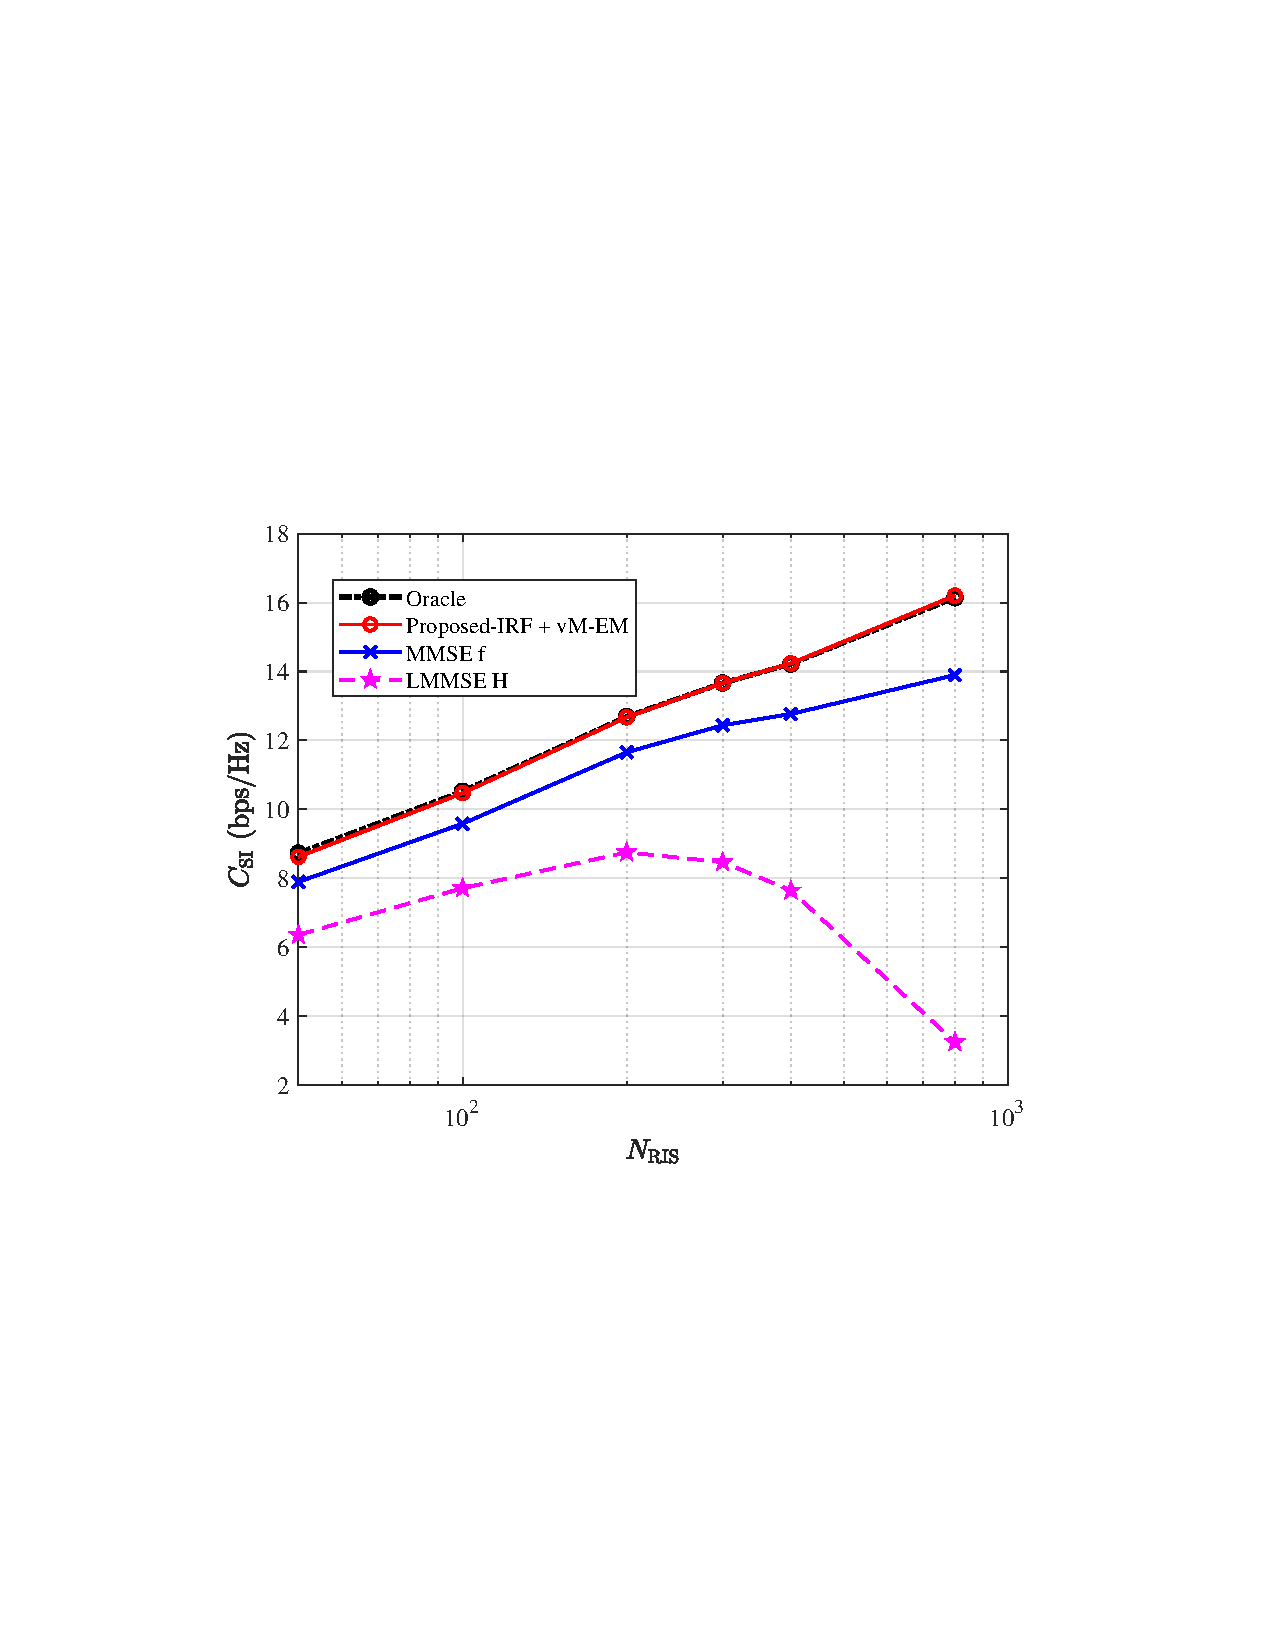
\includegraphics[width=0.7\textwidth]{figs/C-wrt-N_RIS.pdf}
    \caption{Comparison of the capacity upper bound $C_{\rm PSI}$ as a function of the RIS size $N$, where $M=8$. The definition of $C_{\rm PSI}$ will be explained in detail in response to question (6). }
    \label{fig:RIS_size}
\end{figure}

The simulation results are presented in {Fig.~\ref{fig:RIS_size}}. The black dashed Oracle line is obtained by assuming perfect knowledge about both the channel matrices $\bm G$ and $\bm f$; The red line represents the proposed IRF-based CSI acquisition scheme with known $\bm G$ and unknown $\bm f$; The MMSE-$\bm f$ baseline assumes the same channel knowledge as the proposed scheme, but calculates an MMSE estimation for $\bm f$ based on received uplink pilots at the BS; The LMMSE-$\bm H$ scheme assumes no prior channel knowledge. All these curves are drawn with respect to various RIS sizes $N$ ranging from $50$ to $800$. Note that the detailed values $N_y$ and $N_z$ of the planar RIS array are not important, since the i.i.d. Rayleigh fading channel is spatially unstructured.  

It can be derived from {Fig.~\ref{fig:RIS_size}} that, our proposed IRF-based scheme outperforms both of the MMSE schemes, and achieves near-optimal performance within a wide range of RIS sizes. The performance gain is mainly due to the reduced pilot overhead, since as the number of RIS element increases, the pilot overhead of the MMSE-based schemes scales linearly w.r.t. $N$, causing a proportional decrease in the average ergodic capacity per symbol $C_{\rm PSI}$. In the case $N\uparrow B=1000$ for LMMSE-$\bm H$ scheme, the capacity value even starts to drop significantly. However, the proposed IRF scheme does not subject to this capacity reduction, because the overhead is dimension-independent.  


3.3) The reviewer is concerned about the possible inefficiency of the proposed IRF-based RIS channel estimation method in the high sensor noise regime. It is true that if the sensor noise $\sigma_v^2$ is sufficiently large, then it is hard for the proposed IRF-based scheme to obtain any CSI knowledge. And usually, the low-cost power sensors are more noisy than the RF chain receivers. In order to penalize the accuracy of the cost-efficient sensors, we have manually injected more noise into the sensors by setting an additional sensor noise factor $F_p=10\,{\rm dB}$ and an enlarged sensor bandwidth $100\,{\rm MHz}$. The sensor noise is calculated according to 
\begin{equation*}
    \sigma_v^2 = F_p \times {\rm BW}_{\rm sensor}\, n_0,
\end{equation*}
where the thermal noise power spectral density is fixed to $n_0 =-174\,{\rm dBm/Hz}$. As a result, in our simulations, the sensor is set to be $F_p \times {\rm BW}_{\rm sensor}/{\rm BW}_{\rm RF} = 64.9\,{\rm dB}$ noisier than an RF-chain receiver. Even with this unfavorable situation, the IRF-based scheme still outperforms the traditional MMSE-based schemes, because of the {\it double-fading} effect [R6] of the reflective link will highly attenuates the reflective signal during traditional channel estimation. Note that the typical path loss at a distance of $100\,{\rm m}$ is $83.3\,{\rm dB}$ at $3.5\,{\rm GHz}$, and the {\it double-fading} effect doubles this number. 

[R6] M. Najafi, V. Jamali, R. Schober, and H. V. Poor, ``Physics-based modeling and scalable optimization of large intelligent reflecting surfaces,'' {\it IEEE Trans. Commun.}, vol. 69, no. 4, pp. 2673-2691, Apr. 2021.

}}


\textbf{Reviewer 1:}
4) It is not clear how BS beamforming vector $\bm w$ and user's scaler $w'$ are initialized in the proposed algorithms.

{\color{blue}{\textbf{Authors: } 
Thanks for pointing out this very important issue in our paper. We will try to answer this question in two parts. 

4.1) Scalers $\bm w$ and $w'$ during CSI acquisition. In our proposed IRF-based CSI acquisition algorithms, since the user's scaler $w'$ is introduced for the sake of symmetry with the BS's beamformer $\bm w$, it is always assumed that $w'\in\mathbb{R}_+$ equals the square root of the user's pilot transmit power, i.e., $w'$ is fixed to $\sqrt{P_{{\rm u}, p}}$, as is introduced in detail in~\eqref{eqn:transmit_power}. 
For our proposed IRF-based CSI acquisition algorithms, by assuming known BS-RIS link $\bm G$, a sub-optimal solution for $\bm w$ can be obtained by maximizing the total energy that the RIS receives during the creation of IRF, i.e., 
\begin{equation}
    {\bm w}_{\rm IRF} = \underset{\left\|{\bm w}\right\|\leq P_{{\rm BS}, p}}{\rm argmax}\left\|{\bm G}{\bm w} \right\|^2. 
    \label{eqn:IRF_w_opt}
\end{equation}
The solution to~\eqref{eqn:IRF_w_opt} is given by computing the singular value decomposition (SVD) ${\bm G} = {\bm U}{\bm S}{\bm V}\H$, sorting the diagonal entries of $\bm S$ in descending order, and setting ${\bm w}_{\rm IRF} = \sqrt{P_{{\rm BS}, p}}{\bm V}_{(:,1)}$, where ${\bm V}_{(:,1)}$ is the $1^{\rm st}$ column of the matrix ${\bm V}\in\mathbb{C}^{M\times M}$. 
Note that although the solution ${\bm w}_{\rm IRF}$ is a sub-optimal solution, it can still achieve nearly optimal spectral efficiency performance, which is demonstrated by our simulation results.  

4.2) Scalers $\bm w$ and $w'$ during downlink beamforming. For downlink transmission of a MISO system, the user's scaler $w'$ is dummy, so we only consider the BS's beamformer $\bm w$. In our proposed IRF-based method, after the CSI acquisition and the passive RIS beamforming, the BS's active beamformer is adjusted according to~\eqref{eqn:IRF_w_opt}. 
In contrast to this sub-optimal solution~\eqref{eqn:IRF_w_opt}, in the MMSE baselines, the BS's beamformer $\bm w$ is iteratively updated by exploiting the knowledge of the estimated channel $\hat{\bm H}$ according to the following two formulas
\begin{equation}
    \left\{\begin{aligned}
        & {\bm \theta}^{(t+1)} = \exp(-\ri \arg(\hat{\bm H}{\bm w}^{(t)})), \\
        & {\bm w}^{(t+1)} = {\rm norm}(\hat{\bm H}\H {\bm \theta}^{(t+1)*}),
    \end{aligned}\right.
\end{equation}
where ${\bm w}^{(0)}$ is randomly initialized such that $\|{\bm w}^{(0)}\| = \sqrt{P_{{\rm BS}, p}}$. Note that even if our proposed method employs a sub-optimal BS's beamformer $\bm w$, it still outperforms the baselines in terms of the achievable ergodic rate $C_{\rm PSI}$. 

In the revised paper, we have clarified the initialization and updating methods of the BS beamformer ${\bm w}$ and the user's scaler $w'$ for our proposed algorithms as well as the baselines, which is shown as follows.  
\begin{framed}\red{
    Moreover, for the IRF methods, the BS beamformer $\bm w$ is chosen to be the right singular vector that corresponds to the most significant singular value of the BS-RIS channel $\bm G$, which automatically maximizes the total signal energy received by the RIS from the BS, i.e., 
    \begin{equation*}
        {\bm w} = \underset{\left\|{\bm w}\right\|\leq P_{{\rm BS}, p}}{\rm argmax}\left\|{\bm G}{\bm w} \right\|^2,
    \end{equation*}
    and the user's transmit scaler is set to the maximum allowed power $w'=\sqrt{P_{{\rm u}, p}}$ for all the CSI acquisition schemes to ensure a high SNR. 
    For the LMMSE algorithms, after the channel estimation procedure, the beamforming step is fulfilled by alternately updating the BS beamformer $\bm w$ and the RIS phase-shift matrix $\bm\Theta = {\rm diag}({\bm \theta})$ according to  
    \begin{equation*}
        \left\{\begin{aligned}
            & {\bm \theta}^{(t+1)} = \exp(-\ri \arg(\hat{\bm H}{\bm w}^{(t)})), \\
            & {\bm w}^{(t+1)} = \sqrt{P_{{\rm BS}, d}}{\rm norm}(\hat{\bm H}\H {\bm \theta}^{(t+1)*}),
        \end{aligned}\right.
    \end{equation*}
    where ${\rm norm}({\bm z})$ denotes ${\bm z}/\left\|{\bm z}\right\|$. The initial values ${\bm w}^{(0)}$ and ${\bm\theta}^{(0)}$ are generated randomly, and both subject to their corresponding power constraint and unit-modulus constraint, respectively. In our simulations, the iteration is performed at most $T=10$ times. 
}
\end{framed}
}}



\textbf{Reviewer 1:}
5) It would be helpful to incorporate the number of time slots for channel estimation into {\bf Table I}.

{\color{blue}{\textbf{Authors: } 
Thanks for the suggestion of explicitly specifying the number of time slots for channel estimation in {\bf Table I}. In the revised paper, in order to clearly explain the pilot overhead of different schemes, we have changed the overhead index from ``Minimum pilot overhead'' to ``Minimum pilot overhead per user''. We have also clarified in the revised version that, the pilot overhead is equivalent to the number of time slots for channel estimation. Detailed revisions are shown as in the following box: 

\begin{framed}
\red{
    {\bf Table~1} compares the pilot overhead of our proposed IRF method with other different CSI acquisition methods. 
    All the CSI acquisition methods that appear in {\bf Table~1} assume a narrowband system, so the pilot overhead is equal to the number of pilot time slots.
    $K$ denotes the number of users, $S$ is the sparsity of the channel assumption, $M$ is the number of antennas at BS, and $\alpha$ is the ratio of the large-timescale channel  coherence time and the small-timescale channel coherence time [11]. 
    Except for CS-based methods [5], all the channel estimation methods [11], [13], [25] require the pilot overhead to be linearly dependent on $N$, while our IRF method needs a constant number of exactly 3 pilot slots per user, regardless of the number of RIS elements. 
}
\end{framed}
}}

\textbf{Reviewer 1:}
6) Fig.~8 $y$ axis is marked as capacity. However, it is understood that we only know the bound as in [R1]. It would be helpful to present the equations for capacity analysis.

[R1] A. Lapidoth and S. Shamai, ``Fading channels: how perfect need "perfect side information" be?,'' {\it IEEE Trans. Inf. Theory}, vol. 48, no. 5, pp. 1118-1134, May 2002. 

{\color{blue}{\textbf{Authors: } 
Many thanks to the reviewers for their comments on improving the strictness of this paper. In order to specify which capacity formula we employ in this paper, we first introduce the overall procedure of establishing a RIS-aided link. Specifically, we assume that the data transmission is preceded by three link establishment steps:
\begin{enumerate}
    \item Acquire the CSI (apply LMMSE or proposed IRF-based schemes), consuming $N_p$ time slots;
    \item Calculate BS's beamformer $\bm w$ and RIS's phase-shifts $\bm\Theta$ to maximize the user's received signal energy;
    \item Re-estimate the channel, assuming no additional pilot overhead.
\end{enumerate}
The step (3) is needed in real-world systems, because it is very possible that the equivalent BS-RIS-user channel ${\bm f}\H{\bm \Theta}{\bm G}{\bm w}\in\mathbb{C}$ changes significantly after the RIS reconfiguration and the BS beamforming. These changes are not perfectly predictable by previous CSI knowledge due to inaccurate RIS phase-shifts, phase-dependent reflective gain and imprecise BS beamforming. As a result, we assume that a perfect additional channel estimation step (3) is executed after the BS-RIS joint beamforming, and provides perfect CSI in the following data transmission. Since in this paper, we foucs on how to obtain CSI in step (1) for BS active beamforming and RIS passive beamforming in step (2), the pilot overhead for the re-estimation step (3) is omitted. This approximation is reasonable in that only one equivalent channel coefficient needs to be estimated in this step, which is much smaller compared to $NM$ coefficients involved in step (1). 

With this perfect CSI knowledge (side information) in step (3), we consider a block-fading channel with blocklength $B$. Within the same block, the random BS-RIS channel matrix $\bm G$ and the RIS-user channel vector ${\bm f}^*$ are realized for only once. After setting $\bm w$ and $\bm\Theta$ according to steps (1-2), the user's downlink SNR 
\begin{equation}
    \gamma_{\rm user} = \frac{P_{{\rm BS}, d} |{\bm f}\H {\bm \Theta} {\bm G}{\bm w}|^2}{\sigma_z^2}
\end{equation}
determines the ergodic channel capacity within the following $N_d = B-N_p$ data symbols. Thus, the ergodic capacity per channel use is given by 
\begin{equation}
    C_{\rm PSI} = \frac{N_d}{B} \mathbb{E}\left[\log\left( 1+\gamma_{\rm user} \right)\right], \label{eqn:capacity_def}
\end{equation} 
where the subscript PSI indicates that perfect side information [R1] is assumed after the establishment of the RIS-aided reflective link. In our simulations, the expectation in~\eqref{eqn:capacity_def} is numerically approximated by applying the Monte Carlo method. But rigorously speaking, the value $C_{\rm PSI}$ is an upper bound of the true channel capacity of the RIS-aided communication system. 


}}

{\color{blue}{\textbf{Authors: } 
Many thanks again for your valuable time and efforts to review this paper. 

Sincerely, \\
{\it The Authors }
}}

\clearpage

%%%%%%%%%%%%%%%%%%%%%%%%%%%%%%%%%%%%%%%%%%%%%%%%%%%%%%%%%%%%%%%%%%%%%%%%%%%%%%%%%%%%%
%%%%%%%%%%%%%%%%%%%%%%%%%%%%%%%%%%%%%%%%%%%%%%%%%%%%%%%%%%%%%%%%%%%%%%%%%%%%%%%%%%%%%
%%%%%%%%%%%%%%%%%%%%%%%%%%%%%%%%%%%%%%%%%%%%%%%%%%%%%%%%%%%%%%%%%%%%%%%%%%%%%%%%%%%%%
%%%%%%%%%%%%%%%%%%%%%%%%%%%%%%%%%%%%%%%%%%%%%%%%%%%%%%%%%%%%%%%%%%%%%%%%%%%%%%%%%%%%%

\begin{center}
    {\Large\bf Response to Reviewer 2's Comments}
\end{center}

\textbf{Reviewer 2:}
In this paper, the authors propose a dimension-independent channel state information (CSI) acquisition approach for reflecting intelligent surfaces (RIS) in which the required pilot overhead is independent of the number of RIS elements. The main idea is to estimate CSI based on received power variations when both the BS \& user simultaneously transmit to the RIS.

{\color{blue}{\textbf{Authors: } 
We appreciate the reviewer's concise summary of the key points of this paper. We have tried our best to revise the paper according to the reviewer's valuable comments, and our responses are provided in a point-to-point manner as below. 
}}


\textbf{Reviewer 2:}
While the proposed idea \& results seem correct, I do not believe the main contributions of the paper (largely algorithmic) are a good fit for IEEE Transactions on Information Theory. My recommendation to the authors would be to submit the paper to wireless communication- and/or signal processing-focused journals, which would be a better fit for the paper's contributions.

{\color{blue}{\textbf{Authors: } 
Much thanks for the reviewer's positive attitude on the novelty and correctness of this paper. Also, as is stressed by the reviewer, the previous version of this paper lacks a series of sound information-theoretic analyses. We agree with the reviewer that the analytical results are necessary for the high-quality journals like IEEE T-IT. To this end, we have tried our best to provide achievable bounds for our proposed interference random field (IRF)-based CSI acquisition schemes. These newly-added theorems and lemmas are mainly related to detection and estimation theory, which may match the broader scope of this journal. For you to check, we have provided the theoretical contents as follows with some slight modifications, e.g., the number of equations and lemmata may be different from those in the revised paper. 
\begin{framed}
\red{
    \begin{theorem}[MSE of the vM-EM estimator] \label{thm:asymp_perf_vM-EM}
        Assume $\alpha>\beta>0$ are fixed. Then, there exists a sufficiently large integer $L_0$, such that for any $L\geq L_0$, if the proposed vM-EM algorithm converges, the returned estimator $\hat{\varphi}$ achieves an MSE performance of $\mathbb{E}[(\hat{\varphi}-\varphi)^2] = \mathcal{O}(\bar{\gamma}^{-1})$, where $\varphi$ is the true parameter, and $\bar{\gamma}$ is the interferential SNR defined as $\bar{\gamma} = (\alpha^2+\beta^2)/\sigma_v^2$.    
    \end{theorem}
}

    \red{Before proving this theorem, we first introduce the following {\bf Lemma~\ref{lemma:wirtinger_der_vM-EM}} that characterizes how the vM-EM estimator $\hat{\varphi}$ in {\bf Algorithm~2} varies with the random noise vector $\bm v$. }

    \red{\begin{lemma} \label{lemma:wirtinger_der_vM-EM}
        Suppose that for the input data sequence ${\bm s} = \sqrt{{\bm P}/A} = (s_0, \cdots, s_{L-1})\T$, the vM-EM algorithm converges to the estimator $\hat{\varphi}$. Then, the estimator $\hat{\varphi} = \hat{\varphi}({\bm v})$ can be viewed as a function of the noise $\bm v$, and the Wirtinger derivative of $\hat{\varphi}$ w.r.t. $\bm v$ satisfies 
        \begin{equation}
            \|\nabla_{\bm v}\hat{\varphi}\|^2 = \frac{1}{|\langle {\bm s}, {\bm x}\rangle|^2}\sum_{\ell=0}^{L-1}  \frac{\sin^2(\theta_\ell)}{|\mu_\ell|^2}, 
        \end{equation} 
        where ${\bm x} = (x_0, \cdots, x_{L-1})\T$ is defined as 
        \begin{equation}
            x_{\ell} := \frac{(\alpha+\beta \cos\theta_\ell)(\beta+\alpha\cos\theta_\ell)}{|\mu_\ell|^3},~~\ell\in\{L\}, 
        \end{equation}
        and 
        \begin{equation}
            \begin{aligned}
                \mu_\ell & := \alpha+\beta {\rm exp}(\ri \theta_\ell),~~\ell\in\{L\}, \\
                \theta_\ell & := \psi_\ell + \hat{\varphi}, ~~\ell\in\{L\}. 
            \end{aligned}
        \end{equation}
    \end{lemma}
    \begin{IEEEproof}
    The proof is provided in {\bf Appendix E}. 
    \end{IEEEproof}
    }
    
    \red{The aim of {\bf Lemma~\ref{lemma:wirtinger_der_vM-EM}} is to establish the connection between the vM-EM estimator $\hat{\varphi}$ and the noise vector ${\bm v}$. In the following, we denote the estimation error as 
    \begin{equation}
        \Delta\varphi := \hat{\varphi} - \varphi. 
    \end{equation}
    Specifically, it is justified in {\bf Lemma~\ref{lemma:wirtinger_der_vM-EM}} that, the squared error $|\Delta\varphi|^2$ of the vM-EM estimator is intrinsically bounded by the noise energy $\|{\bm v}\|^2$, since the differential ${\rm d}\Delta\varphi$ of a general complex-valued function $\Delta\varphi: \mathbb{C}\to\mathbb{C}$ can be written as 
    \begin{equation}
        {\rm d}\Delta\varphi = \langle \nabla_{\bm v}\hat{\varphi}, {\rm d}{\bm v}^*\rangle + \langle \nabla_{{\bm v}^*}\hat{\varphi}, {\rm d}{\bm v}\rangle, 
    \end{equation}
    where for real-valued function $\hat{\varphi}({\bm v}): \mathbb{C}^L \to [0,2\pi]\subset \mathbb{R}$ this differential relation reduces to 
    \begin{equation}
        {\rm d}\Delta\varphi = 2\Re\langle\nabla_{\bm v}\hat{\varphi}, {\rm d}{\bm v}^*\rangle. 
        \label{eqn:differential_of_error}
    \end{equation}
    Thus, an integration inequality will hold to upper-bound the MSE of the estimator $\hat{\varphi}$, i.e., 
    \begin{equation}
        \begin{aligned}
            |\Delta{\varphi}|^2 &= \left| \int {\rm d}\Delta\varphi \right|^2 \\
            &= 4 \left| \int_{0}^{1} \Re\langle\nabla_{{\bm v}'=t {\bm v}}\hat{\varphi}, {\bm v}\rangle{\rm d}t \right|^2 \\
            &\leq 4\|{\bm v}\|^2 \left(\int_{0}^{1} \|\nabla_{{\bm v}'=t{\bm v}}\hat{\varphi} \| {\rm d} t \right)^2. 
        \end{aligned}
        \label{ineq:gradient_bound}
    \end{equation}
    Before explaining this idea in detail, we first introduce some interesting results about some intermediate variables. }
    
    \red{\begin{lemma}[Asymptotic invariants]\label{lemma:asymp_inv}
        Suppose $\alpha > \beta > 0$. If we define 
        \begin{equation}
            \begin{aligned}
                H_L & :=\frac{1}{L}\sum_{\ell=0}^{L-1} \frac{\sin^2(\theta_\ell)}{|\mu_\ell|^2}, \\
                G_L & := \frac{1}{L}\sum_{\ell=0}^{L-1} \frac{(\alpha+\beta \cos(\theta_\ell))(\beta+\alpha\cos(\theta_\ell))}{|\mu_\ell|^2}, \\
            \end{aligned}
        \end{equation}
        then the sequences $H_L$ and $G_L$ are intrinsically independent of the estimator $\hat{\varphi}\in[0,2\pi]$ as $L\to\infty$. Specifically, 
        \begin{equation}
            \begin{aligned}
                H &= H_{\infty} + \mathcal{O}(L^{-1}), \\
                G &= G_{\infty} + \mathcal{O}(L^{-1}), 
            \end{aligned}
        \end{equation}
        where 
        \begin{equation}
            \begin{aligned}
                H_{\infty} &=  \frac{1}{2\pi}\int_{0}^{2\pi} \frac{\sin^2\theta}{\alpha^2+\beta^2+2\alpha\beta\cos(\theta)}{\rm d}\theta = \frac{1}{2\alpha^2},  \\
                G_{\infty} &= \frac{1}{2\pi}\int_{0}^{2\pi} \frac{(\alpha+\beta\cos(\theta))(\beta+\alpha\cos(\theta))}{\alpha^2+\beta^2+2\alpha\beta\cos(\theta)} {\rm d}\theta = \frac{\beta}{2\alpha}.  \\ 
            \end{aligned}
        \end{equation}
    \end{lemma}
    }
    
    
    \red{{\it Proof Sketch.} The integral expressions for $H_\infty$ and $G_\infty$ as well as the asymptotic remainders $\mathcal{O}(L^{-1})$ can be obtained by applying the numerical trapezoidal integration formula to the definition of the sequence $H_L$ and $G_L$. The integrals on $[0,2\pi]$ can be evaluated by the following replacements:
    \begin{equation}
        \begin{aligned}
            & {\rm d}\theta  \to \frac{\d z}{\ri z}, & \int_0^{2\pi} \to \int_{|z|=1}, \\
            & \sin\theta  \to \frac{z-z^{-1}}{2\ri}, & \cos\theta \to \frac{z+z^{-1}}{2}, \\
        \end{aligned}
    \end{equation}
    and the applying the Residue Theorem to all poles inside the closed curve $|z|=1$. }
    
    \red{\begin{remark}
        These limiting expressions will play an important rule in obtaining the upper bound of the estimation error $|\Delta\varphi|$, since this invariance can asymptotically eliminate the dependency of the Wirtinger derivative ({\bf Lemma~\ref{lemma:wirtinger_der_vM-EM}}) on the unknown estimator $\hat{\varphi}$. 
    \end{remark}}
    
    \red{\begin{remark}
        In fact, we can also prove that 
        \begin{equation}
            \frac{\|{\bm x}\|^2}{L} = \frac{2\alpha^2-\beta^2/2}{4\alpha^2(\alpha^2-\beta^2)} + \mathcal{O}(L^{-1}),~~\alpha>\beta>0
        \end{equation}
        by the same numerical integration approximation technique and the Residue Theorem. 
    \end{remark} }
    
    
    \red{\begin{lemma}[ODE bound] \label{lemma:ODE-bound}
        Suppose for the input data sequence ${\bm s} = \sqrt{{\bm P}/A} = (s_0, \cdots, s_{L-1})\T$, the vM-EM algorithm converges, and the estimation error is denoted by $\Delta\varphi = \hat{\varphi} - \varphi$. Then, for any sufficiently large $L\geq L_0$, there exists some positive $\delta = \delta(L)>0$ and $C=C(L)>0$, such that for any noise vector ${\bm v}$ satisfying $\|{\bm v}\|/\sqrt{L} \leq \delta$, the estimation error is upper-bounded by
        \begin{equation}
            |\Delta\varphi|\leq C \frac{\|{\bm v}\|}{\sqrt{L}}. 
        \end{equation}
    \end{lemma}
    \begin{IEEEproof}
        The proof is provided in {\bf Appendix~F}. 
    \end{IEEEproof}
    From the above {\bf Lemma~\ref{lemma:ODE-bound}}, we can directly prove {\bf Theorem~\ref{thm:asymp_perf_vM-EM}}. Choose $L\geq L_0$, and then let us compute the MMSE of the vM-EM estimator, i.e., 
    \ifx\onecol\undefined
    \begin{equation}
        \begin{aligned}
        \mathbb{E}[(\hat{\varphi}-\varphi)^2] &= \mathbb{E}[|\Delta\varphi|^2] \\
        &= \mathbb{E}\left[|\Delta\varphi|^2 \Bigg|\frac{\|{\bm v}\|}{\sqrt{L}} \leq \delta \right]\mathbb{P}\left[\frac{\|{\bm v}\|}{\sqrt{L}} \leq \delta \right] \\
        & + \mathbb{E}\left[|\Delta\varphi|^2 \Bigg|\frac{\|{\bm v}\|}{\sqrt{L}} > \delta \right]\mathbb{P}\left[\frac{\|{\bm v}\|}{\sqrt{L}}>\delta \right] \\
        & \leq C^2 \mathbb{E}\left[\frac{\|{\bm v}\|^2}{L}\right] + \pi^2 \mathbb{P}\left[\frac{\|{\bm v}\|}{\sqrt{L}}>\delta\right] \\
        & \overset{(a)}{\leq} C^2\sigma_v^2 + \pi^2 \frac{\mathbb{E}\left[\left(\frac{\|{\bm v}\|}{\sqrt{L}}\right)^r\right]}{\delta^r},
        \end{aligned}
    \end{equation}
    \else 
    \begin{equation}
        \begin{aligned}
        \mathbb{E}[(\hat{\varphi}-\varphi)^2] &= \mathbb{E}[|\Delta\varphi|^2] \\
        &= \mathbb{E}\left[|\Delta\varphi|^2 \Bigg|\frac{\|{\bm v}\|}{\sqrt{L}} \leq \delta \right]\mathbb{P}\left[\frac{\|{\bm v}\|}{\sqrt{L}} \leq \delta \right] + \mathbb{E}\left[|\Delta\varphi|^2 \Bigg|\frac{\|{\bm v}\|}{\sqrt{L}} > \delta \right]\mathbb{P}\left[\frac{\|{\bm v}\|}{\sqrt{L}}>\delta \right] \\
        & \leq C^2 \mathbb{E}\left[\frac{\|{\bm v}\|^2}{L}\right] + \pi^2 \mathbb{P}\left[\frac{\|{\bm v}\|}{\sqrt{L}}>\delta\right] \\
        & \overset{(a)}{\leq} C^2\sigma_v^2 + \pi^2 \frac{\mathbb{E}\left[\left(\frac{\|{\bm v}\|}{\sqrt{L}}\right)^r\right]}{\delta^r},
        \end{aligned}
    \end{equation}
    \fi
    where (a) comes from applying the Markov inequality, and $r>0$ can be arbitrarily chosen. Particularly, by setting $r=2$, we obtain 
    \begin{equation}
        \mathbb{E}\left[(\hat{\varphi} - \varphi)\right] \leq \sigma_v^2(C^2+\pi^2/\delta^2) = \mathcal{O}(\bar{\gamma}^{-1}),  
    \end{equation}
    which completes the proof of {\bf Theorem~\ref{thm:asymp_perf_vM-EM}}.  }
    
    \red{\begin{remark}
        The conclusion of {\bf Theorem~\ref{thm:asymp_perf_vM-EM}} guarantees that as $\bar{\gamma}\to\infty$, the MSE of the vM-EM estimator decays at a rate of at least $(\bar{\gamma})^{-1}$. This conclusion is verified in the following numerical simulation, where it is shown that the MSE curve of the proposed vM-EM algorithm has an asymptotic slope of $-1$ in the logarithmic coordinate. 
    \end{remark} }
    
\end{framed}


The newly-added proofs of the above lemmas and theorems are provided in the revised paper. 
}}

{\color{blue}{\textbf{Authors: } 
Many thanks again for your valuable time and efforts to review this paper. 

Sincerely, \\
{\it The Authors }
}}

\clearpage 

%%%%%%%%%%%%%%%%%%%%%%%%%%%%%%%%%%%%%%%%%%%%%%%%%%%%%%%%%%%%%%%%%%%%%%%%%%%%%%%%%%%%%
%%%%%%%%%%%%%%%%%%%%%%%%%%%%%%%%%%%%%%%%%%%%%%%%%%%%%%%%%%%%%%%%%%%%%%%%%%%%%%%%%%%%%
%%%%%%%%%%%%%%%%%%%%%%%%%%%%%%%%%%%%%%%%%%%%%%%%%%%%%%%%%%%%%%%%%%%%%%%%%%%%%%%%%%%%%
%%%%%%%%%%%%%%%%%%%%%%%%%%%%%%%%%%%%%%%%%%%%%%%%%%%%%%%%%%%%%%%%%%%%%%%%%%%%%%%%%%%%%


\begin{center}
    {\Large\bf Response to Reviewer 3's Comments}
\end{center}

\textbf{Reviewer 3:}
This paper introduces a dimension-independent CSI acquisition method for sensing
RIS-assisted MISO wireless communication systems. The key issue of the paper is that the achievable schemes look like heuristic with no performance guarantees, and the methodology does not seem novel.

{\color{blue}{\textbf{Authors: } 
We appreciate the reviewer's concise summary of the key points of this paper. We have tried our best to address these issues in the revised paper according to the reviewer's valuable comments. Specifically, we have proved achievable theorems for our proposed vM-EM phase estimation algorithm, and our responses are provided in a point-to-point manner as below. 
}}

\textbf{Reviewer 3:}
1) The paper considers a MISO system. Can the approaches work for MIMO system?

{\color{blue}{\textbf{Authors: } 
Thanks for the insightful comments of the reviewer. Since the definition of MIMO systems usually include two possible explanations: the multi-antenna MIMO and the multi-user MIMO, we will elaborate on both of these two explanations. 

1.1) Actually, the extensibility to multi-antenna MIMO case is possible without sacrificing the number of time slots for CSI acquisition. By placing the pilot symbols on different OFDM subcarriers across different antennas, all the antennas at the user can transmit rotational pilots simultaneously at different frequencies. Then, the power sensors attached to each RIS element can split the interference random field (IRF) signal into components of different frequencies and perform phase estimation separately for different antennas. Mathematically, it is possible to retrieve $K$ different phases $\varphi_k\in[0,2\pi], k\in\{1,2,\cdots,K\}$ from the following composite power signal 
\begin{equation}
    P(t) = \left|\alpha + \sum_{k=1}^{K} \beta_k e^{\ri \omega_k t}  e^{\ri \varphi_k}\right|^2,
\end{equation}
where $\beta_k>0$, and $\omega_k\neq\omega_\ell$ for different antenna indices $k,\ell$. In fact, by assuming a sufficiently small interferential power ratio $r=(\alpha)^{-2}\sum_k \beta_k^2$, the above power signal can be locally linearized into one DC component $\alpha^2$ and $K$ AC components of different frequencies, which may further be separated by directly applying the Fourier transform. Clearly, this sensing RIS-aided multi-antenna MIMO CSI acquisition method is sub-optimal. However, designing the optimal method to estimate all the $\varphi_k$ and $\beta_k$ accurately is also interesting, and we will leave it for our future work. 

1.2) The extensibility to multi-user MIMO case. Similar to the above multi-antenna MIMO case, the simultaneous CSI acquisition methodology also works for the multi-user case. By transmitting pilot symbols that rotate at different frequencies, the RIS power sensor can still distinguish between different users. 
Moreover, since usually different users are separated in the angular domain from the RIS's perspective [R1], in the multi-user case, the RIS can further exploit such angular separation property to distinguish between different users. Thus, by exploiting multi-sensor joint detection and estimation at the RIS, the CSI acquisition precision may be further improved. Such an extension to the multi-user MIMO case is also left for our future work, and we have added a brief discussion about this idea in the revised version.  

% It is worth pointing out that the method we proposed to estimate the channel phase difference $\varphi$ is heuristic, which may not be the optimal one. It has been verified in the paper that our method is simple and efficient. However, designing the optimal method to estimate ${{\varphi_{l,c}}}$ is also interesting, and we will leave it for our future work. In the revised paper, we have addressed this issue as:

Specifically, in the revised paper, we have addressed these issues as:

\begin{framed}
    \red{In fact, for multi-antenna MIMO systems, rotating pilot symbols at different frequencies $k$ can be simultaneously transmitted by different antennas to enable CSI acquisition.  
    Then, the multi-antenna CSI acquisition can be fulfilled by performing Fourier analysis on the composite IRF power signal $P(t)$, and extracting the phase angles for each antenna at distinct frequencies. 
    Similarly, this pseudo-frequency division idea can be extended to multi-user MIMO systems, where different users can also be distinguished by different IRF frequencies. Fortunately, since different users are usually separated in the angular domain from the RIS's perspective, these users can be further identified by performing joint detection and estimation across all the RIS sensors. The joint CSI estimation is beyond the scope of this paper, and is left for our future work. }
\end{framed}


[R1] C. Pan et al., ``An Overview of Signal Processing Techniques for RIS/IRS-Aided Wireless Systems,'' {\it IEEE J. Sel. Topics Signal Process.}, vol. 16, no. 5, pp. 883-917, Aug. 2022. 


}}

\textbf{Reviewer 3:}
2) The new contribution from algorithm seems to be phase estimation in Section V. However, all the approaches seem direct and heuristic. There are no performance guarantees of the proposed approaches.

{\color{blue}{\textbf{Authors: } 
Many thanks for the reviewer's high expectation on this paper. To respond to the reviewer's questions, we would like to clarify our contributions and explain the meanings of the proposed algorithms in a more systematic manner. 
Specifically, we will show the underlying logic in the proposed algorithms to justify their rationale. 
Also, as is stressed by the reviewer, it is important to provide performance guarantees for the proposed approaches. We have tried our best to conceive some theorems on the achievability of our proposed algorithms, and the performance guarantees will be provided in response to {\bf question 3)}, which will be presented later. 

We would like to commence by elaborating the novelty of the proposed methods. In this paper, we have proposed a new approach for CSI acquisition by exploiting the power detection capability of sensing RIS. This approach is fundamentally different from the existing schemes in that: 
\begin{enumerate}
    \item The proposed CSI acquisition scheme is performed at the RIS instead of the baseband processors at the receivers. Since no RF chains are equipped at the RIS, it seems impossible to obtain the phase information of the channels. To attack this problem, we try to exploit the physical phenomenon of interference to convert the hard-to-detect phase information into easy-to-detect intensity information, which finally leads to our idea of creating the interference random field (IRF) for CSI acquisition.  
    \item The proposed IRF-based methods can realize dimension-independent CSI acquisition task in a cost-efficient manner. We have proved in this paper that it is possible to acquire enough CSI for accurate beamforming in only 3 pilot slots, without requiring too much hardware cost. It is true that dimension-independent CSI acquisition can also be realized by attaching an adequate number of RF chains to the RIS's elements [R1-R2], however, we demonstrate that the same near-optimal performance can be achieved by adding only cost-efficient power sensors, which are usually much cheaper than RF chains [R3] and much easier to be integrated onto the RIS's microwave structure [R4]. 
\end{enumerate}

After proposing the concept of sensing RIS and explaining the basic principles of how it works, the remaining task is to construct an efficient algorithm to extract the desired CSI from the observed power signals. Specifically, for the RIS beamforming tasks, it suffices to estimate the phase difference $\varphi_n = \arg(f_n^*) - \arg({\bm g}_n\T {\bm w})$ between the BS-RIS and the RIS-user channels. 
Given the observed sequence $P_\ell = |\alpha + \beta\exp(\ri \psi_\ell)\exp(\ri \varphi) + v_\ell|^2$, our goal is to recover the unknown phase $\varphi$ with the prior knowledge of $\psi_\ell$ in the third pilot slot ($\alpha$ and $\beta$ can be easily estimated from the two preceding pilot slots), leading to the name ``phase estimation''. 

In this paper, we proposed three methods to solve this phase estimation problem. Due to the nonlinear nature of the squaring operation, traditional signal processing techniques including the Fourier spectrum analysis becomes suboptimal. Thus, the first proposed approach, i.e., the DFT method, serves as a suboptimal baseline for all the following proposed schemes. Furthermore, since the probability distributions of the power signals $P_\ell$ are clearly specified (noncentral chi-squared distribution), the ML method is theoretically applicable to this problem. However, the ML method involves intensive evaluations of modified Bessel functions, which is usually computationally intractable on typical RIS microcontrollers. 
Thus, to reduce the computational cost of phase estimation, we construct an expectation-maximization (EM) algorithm that assigns a von Mises prior distribution to $\varphi$, thus it is called the vM-EM algorithm. 
This algorithm regards the noiseless complex signal $\mu_\ell := \alpha+\beta\exp(\ri\psi_\ell)\exp(\ri\varphi)$ as a latent variable depending on the unknown parameter $\varphi$, and works by alternately estimating the latent variables $\mu_\ell$ and the unknown phase $\varphi$. 
Furthermore, the EM steps are carefully designed to preserve the von Mises distribution property of the updated estimator $\hat{\varphi}|\{P_\ell\}$, satisfying the conjugate prior condition [R5] for computational convenience. In our simulation results, the proposed vM-EM algorithm is compared with two baselines: the DFT method and the ML method, and it is demonstrated by the numerical simulation that the vM-EM method can achieve comparable performance with the ML method. 

[R1] G. C. Alexandropoulos and E. Vlachos, ``A hardware architecture for reconfigurable intelligent surfaces with minimal active elements for explicit channel estimation,'' in {\it Proc. IEEE Int. Conf. on Acoust., Speech
and Signal Process. (ICASSP)}, May 2020. 

[R2] E. Vlachos, G. C. Alexandropoulos, and J. Thompson, ``Wideband MIMO channel estimation for hybrid beamforming millimeter wave systems via random spatial sampling,'' {\it IEEE J. Sel. Topics Signal Process.}, vol. 13, no. 5, pp. 1136-1150, 2019.

[R3] Y. Zhou and M. Y.-W. Chia, ``A Low-Power Ultra-Wideband CMOS True RMS Power Detector,'' {\it IEEE Trans. Micro. Theory Techn.}, vol. 56, no. 5, pp. 1052-1058, May 2008. 

[R4] Q. Ma, G. D. Bai, H. B. Jing, C. Yang, L. Li, and T. J. Cui, ``Smart metasurface with self-adaptively reprogrammable functions,'' {\it Light: science \& applications}, vol. 8, no. 1, pp. 1-12, Oct. 2019.

[R5] P. Diaconis and D. Ylvisaker, ``Conjugate Priors for Exponential Families,'' {\it The Annals of Statistics}, vol. 7, no. 2, pp. 269-281, 1979.


}}

\textbf{Reviewer 3:}
3) All the theorems seem to be on CRLB rather than the achievability. As such, the achievable strategy and CRLB comparison will add credibility to the achievability.

{\color{blue}{\textbf{Authors: } 
Many thanks for the reivewer's positive attitude on the correctness of the CRLB. As is pointed out by the reviewer, the theoretical results in the previous version of this paper are mainly focused on the ``converse'' theorems (the CRLB) instead of the ``achievability'' theorems, which does not provide a firm performance guarantee for our proposed schemes. In order to address this concern, we have tried our best to provide theorems on the achievability of the proposed interference random field (IRF)-based CSI acquisition schemes. 

These newly-added theorems and lemmas are mainly related to detection and estimation theory, which may match the broader scope of this journal. For you to check, we have provided the theoretical contents as follows with some slight modifications, e.g., the number of equations and lemmata may be different from those in the revised paper. The detailed proofs are provided in the {\bf Appendices} of the revised paper.  

\begin{framed}
    \red{
        \begin{theorem}[MSE of the vM-EM estimator] \label{thm3:asymp_perf_vM-EM}
            Assume $\alpha>\beta>0$ are fixed. Then, there exists a sufficiently large integer $L_0$, such that for any $L\geq L_0$, if the proposed vM-EM algorithm converges, the returned estimator $\hat{\varphi}$ achieves an MSE performance of $\mathbb{E}[(\hat{\varphi}-\varphi)^2] = \mathcal{O}(\bar{\gamma}^{-1})$, where $\varphi$ is the true parameter, and $\bar{\gamma}$ is the interferential SNR defined as $\bar{\gamma} = (\alpha^2+\beta^2)/\sigma_v^2$.    
        \end{theorem}
    }
    
        \red{Before proving this theorem, we first introduce the following {\bf Lemma~\ref{lemma:wirtinger_der_vM-EM}} that characterizes how the vM-EM estimator $\hat{\varphi}$ in {\bf Algorithm~2} varies with the random noise vector $\bm v$. }
    
        \red{\begin{lemma} \label{lemma3:wirtinger_der_vM-EM}
            Suppose that for the input data sequence ${\bm s} = \sqrt{{\bm P}/A} = (s_0, \cdots, s_{L-1})\T$, the vM-EM algorithm converges to the estimator $\hat{\varphi}$. Then, the estimator $\hat{\varphi} = \hat{\varphi}({\bm v})$ can be viewed as a function of the noise $\bm v$, and the Wirtinger derivative of $\hat{\varphi}$ w.r.t. $\bm v$ satisfies 
            \begin{equation}
                \|\nabla_{\bm v}\hat{\varphi}\|^2 = \frac{1}{|\langle {\bm s}, {\bm x}\rangle|^2}\sum_{\ell=0}^{L-1}  \frac{\sin^2(\theta_\ell)}{|\mu_\ell|^2}, 
            \end{equation} 
            where ${\bm x} = (x_0, \cdots, x_{L-1})\T$ is defined as 
            \begin{equation}
                x_{\ell} := \frac{(\alpha+\beta \cos\theta_\ell)(\beta+\alpha\cos\theta_\ell)}{|\mu_\ell|^3},~~\ell\in\{L\}, 
            \end{equation}
            and 
            \begin{equation}
                \begin{aligned}
                    \mu_\ell & := \alpha+\beta {\rm exp}(\ri \theta_\ell),~~\ell\in\{L\}, \\
                    \theta_\ell & := \psi_\ell + \hat{\varphi}, ~~\ell\in\{L\}. 
                \end{aligned}
            \end{equation}
        \end{lemma}
        \begin{IEEEproof}
        The proof is provided in {\bf Appendix E}. 
        \end{IEEEproof}
        }
        
        \red{The aim of {\bf Lemma~\ref{lemma:wirtinger_der_vM-EM}} is to establish the connection between the vM-EM estimator $\hat{\varphi}$ and the noise vector ${\bm v}$. In the following, we denote the estimation error as 
        \begin{equation}
            \Delta\varphi := \hat{\varphi} - \varphi. 
        \end{equation}
        Specifically, it is justified in {\bf Lemma~\ref{lemma:wirtinger_der_vM-EM}} that, the squared error $|\Delta\varphi|^2$ of the vM-EM estimator is intrinsically bounded by the noise energy $\|{\bm v}\|^2$, since the differential ${\rm d}\Delta\varphi$ of a general complex-valued function $\Delta\varphi: \mathbb{C}\to\mathbb{C}$ can be written as 
        \begin{equation}
            {\rm d}\Delta\varphi = \langle \nabla_{\bm v}\hat{\varphi}, {\rm d}{\bm v}^*\rangle + \langle \nabla_{{\bm v}^*}\hat{\varphi}, {\rm d}{\bm v}\rangle, 
        \end{equation}
        where for real-valued function $\hat{\varphi}({\bm v}): \mathbb{C}^L \to [0,2\pi]\subset \mathbb{R}$ this differential relation reduces to 
        \begin{equation}
            {\rm d}\Delta\varphi = 2\Re\langle\nabla_{\bm v}\hat{\varphi}, {\rm d}{\bm v}^*\rangle. 
            \label{eqn3:differential_of_error}
        \end{equation}
        Thus, an integration inequality will hold to upper-bound the MSE of the estimator $\hat{\varphi}$, i.e., 
        \begin{equation}
            \begin{aligned}
                |\Delta{\varphi}|^2 &= \left| \int {\rm d}\Delta\varphi \right|^2 \\
                &= 4 \left| \int_{0}^{1} \Re\langle\nabla_{{\bm v}'=t {\bm v}}\hat{\varphi}, {\bm v}\rangle{\rm d}t \right|^2 \\
                &\leq 4\|{\bm v}\|^2 \left(\int_{0}^{1} \|\nabla_{{\bm v}'=t{\bm v}}\hat{\varphi} \| {\rm d} t \right)^2. 
            \end{aligned}
            \label{ineq3:gradient_bound}
        \end{equation}
        Before explaining this idea in detail, we first introduce some interesting results about some intermediate variables. }
        
        \red{\begin{lemma}[Asymptotic invariants]\label{lemma3:asymp_inv}
            Suppose $\alpha > \beta > 0$. If we define 
            \begin{equation}
                \begin{aligned}
                    H_L & :=\frac{1}{L}\sum_{\ell=0}^{L-1} \frac{\sin^2(\theta_\ell)}{|\mu_\ell|^2}, \\
                    G_L & := \frac{1}{L}\sum_{\ell=0}^{L-1} \frac{(\alpha+\beta \cos(\theta_\ell))(\beta+\alpha\cos(\theta_\ell))}{|\mu_\ell|^2}, \\
                \end{aligned}
            \end{equation}
            then the sequences $H_L$ and $G_L$ are intrinsically independent of the estimator $\hat{\varphi}\in[0,2\pi]$ as $L\to\infty$. Specifically, 
            \begin{equation}
                \begin{aligned}
                    H &= H_{\infty} + \mathcal{O}(L^{-1}), \\
                    G &= G_{\infty} + \mathcal{O}(L^{-1}), 
                \end{aligned}
            \end{equation}
            where 
            \begin{equation}
                \begin{aligned}
                    H_{\infty} &=  \frac{1}{2\pi}\int_{0}^{2\pi} \frac{\sin^2\theta}{\alpha^2+\beta^2+2\alpha\beta\cos(\theta)}{\rm d}\theta = \frac{1}{2\alpha^2},  \\
                    G_{\infty} &= \frac{1}{2\pi}\int_{0}^{2\pi} \frac{(\alpha+\beta\cos(\theta))(\beta+\alpha\cos(\theta))}{\alpha^2+\beta^2+2\alpha\beta\cos(\theta)} {\rm d}\theta = \frac{\beta}{2\alpha}.  \\ 
                \end{aligned}
            \end{equation}
        \end{lemma}
        }
        
        
        \red{{\it Proof Sketch.} The integral expressions for $H_\infty$ and $G_\infty$ as well as the asymptotic remainders $\mathcal{O}(L^{-1})$ can be obtained by applying the numerical trapezoidal integration formula to the definition of the sequence $H_L$ and $G_L$. The integrals on $[0,2\pi]$ can be evaluated by the following replacements:
        \begin{equation}
            \begin{aligned}
                & {\rm d}\theta  \to \frac{\d z}{\ri z}, & \int_0^{2\pi} \to \int_{|z|=1}, \\
                & \sin\theta  \to \frac{z-z^{-1}}{2\ri}, & \cos\theta \to \frac{z+z^{-1}}{2}, \\
            \end{aligned}
        \end{equation}
        and the applying the Residue Theorem to all poles inside the closed curve $|z|=1$. }
        
        \red{\begin{remark}
            These limiting expressions will play an important rule in obtaining the upper bound of the estimation error $|\Delta\varphi|$, since this invariance can asymptotically eliminate the dependency of the Wirtinger derivative ({\bf Lemma~\ref{lemma:wirtinger_der_vM-EM}}) on the unknown estimator $\hat{\varphi}$. 
        \end{remark}}
        
        \red{\begin{remark}
            In fact, we can also prove that 
            \begin{equation}
                \frac{\|{\bm x}\|^2}{L} = \frac{2\alpha^2-\beta^2/2}{4\alpha^2(\alpha^2-\beta^2)} + \mathcal{O}(L^{-1}),~~\alpha>\beta>0
            \end{equation}
            by the same numerical integration approximation technique and the Residue Theorem. 
        \end{remark} }
        
        
        \red{\begin{lemma}[ODE bound] \label{lemma3:ODE-bound}
            Suppose for the input data sequence ${\bm s} = \sqrt{{\bm P}/A} = (s_0, \cdots, s_{L-1})\T$, the vM-EM algorithm converges, and the estimation error is denoted by $\Delta\varphi = \hat{\varphi} - \varphi$. Then, for any sufficiently large $L\geq L_0$, there exists some positive $\delta = \delta(L)>0$ and $C=C(L)>0$, such that for any noise vector ${\bm v}$ satisfying $\|{\bm v}\|/\sqrt{L} \leq \delta$, the estimation error is upper-bounded by
            \begin{equation}
                |\Delta\varphi|\leq C \frac{\|{\bm v}\|}{\sqrt{L}}. 
            \end{equation}
        \end{lemma}
        \begin{IEEEproof}
            The proof is provided in {\bf Appendix~F}. 
        \end{IEEEproof}
        From the above {\bf Lemma~\ref{lemma:ODE-bound}}, we can directly prove {\bf Theorem~\ref{thm:asymp_perf_vM-EM}}. Choose $L\geq L_0$, and then let us compute the MMSE of the vM-EM estimator, i.e., 
        \ifx\onecol\undefined
        \begin{equation}
            \begin{aligned}
            \mathbb{E}[(\hat{\varphi}-\varphi)^2] &= \mathbb{E}[|\Delta\varphi|^2] \\
            &= \mathbb{E}\left[|\Delta\varphi|^2 \Bigg|\frac{\|{\bm v}\|}{\sqrt{L}} \leq \delta \right]\mathbb{P}\left[\frac{\|{\bm v}\|}{\sqrt{L}} \leq \delta \right] \\
            & + \mathbb{E}\left[|\Delta\varphi|^2 \Bigg|\frac{\|{\bm v}\|}{\sqrt{L}} > \delta \right]\mathbb{P}\left[\frac{\|{\bm v}\|}{\sqrt{L}}>\delta \right] \\
            & \leq C^2 \mathbb{E}\left[\frac{\|{\bm v}\|^2}{L}\right] + \pi^2 \mathbb{P}\left[\frac{\|{\bm v}\|}{\sqrt{L}}>\delta\right] \\
            & \overset{(a)}{\leq} C^2\sigma_v^2 + \pi^2 \frac{\mathbb{E}\left[\left(\frac{\|{\bm v}\|}{\sqrt{L}}\right)^r\right]}{\delta^r},
            \end{aligned}
        \end{equation}
        \else 
        \begin{equation}
            \begin{aligned}
            \mathbb{E}[(\hat{\varphi}-\varphi)^2] &= \mathbb{E}[|\Delta\varphi|^2] \\
            &= \mathbb{E}\left[|\Delta\varphi|^2 \Bigg|\frac{\|{\bm v}\|}{\sqrt{L}} \leq \delta \right]\mathbb{P}\left[\frac{\|{\bm v}\|}{\sqrt{L}} \leq \delta \right] + \mathbb{E}\left[|\Delta\varphi|^2 \Bigg|\frac{\|{\bm v}\|}{\sqrt{L}} > \delta \right]\mathbb{P}\left[\frac{\|{\bm v}\|}{\sqrt{L}}>\delta \right] \\
            & \leq C^2 \mathbb{E}\left[\frac{\|{\bm v}\|^2}{L}\right] + \pi^2 \mathbb{P}\left[\frac{\|{\bm v}\|}{\sqrt{L}}>\delta\right] \\
            & \overset{(a)}{\leq} C^2\sigma_v^2 + \pi^2 \frac{\mathbb{E}\left[\left(\frac{\|{\bm v}\|}{\sqrt{L}}\right)^r\right]}{\delta^r},
            \end{aligned}
        \end{equation}
        \fi
        where (a) comes from applying the Markov inequality, and $r>0$ can be arbitrarily chosen. Particularly, by setting $r=2$, we obtain 
        \begin{equation}
            \mathbb{E}\left[(\hat{\varphi} - \varphi)\right] \leq \sigma_v^2(C^2+\pi^2/\delta^2) = \mathcal{O}(\bar{\gamma}^{-1}),  
        \end{equation}
        which completes the proof of {\bf Theorem~\ref{thm:asymp_perf_vM-EM}}.  }
        
        \red{\begin{remark}
            The conclusion of {\bf Theorem~\ref{thm:asymp_perf_vM-EM}} guarantees that as $\bar{\gamma}\to\infty$, the MSE of the vM-EM estimator decays at a rate of at least $(\bar{\gamma})^{-1}$. This conclusion is verified in the following numerical simulation, where it is shown that the MSE curve of the proposed vM-EM algorithm has an asymptotic slope of $-1$ in the logarithmic coordinate. 
        \end{remark} }
        
    \end{framed}

}}

{\color{blue}{\textbf{Authors: } 
Many thanks again for your valuable time and efforts to review this paper. 

Sincerely, \\
{\it The Authors }
}}


\clearpage 



{\color{blue}{\textbf{Authors}}: We would like to commence by thanking the editor and three professional reviewers for their valuable time in evaluating our submission. Your constructive comments and expert knowledge of the field have helped us to strengthen the manuscript significantly. We endeavored to address all the suggestions and comments, and our reflections are provided below in a point-by-point way. We also indicate how our manuscript has been revised accordingly, and all the revisions have been highlighted in {\color{red} red} color in the revised paper. Here, we would like to make a brief summary of the major revisions in the revised paper as below:

1) We have clarified all the unclear statements pointed out by the reviewers, such as ``why the lens antenna array can realize the spatial DFT" and ``why we design the overall combining matrix ${{{\bf{\bar W}}}}$ as a Bernoulli random matrix".

2) We have justified all impractical assumptions pointed out by the reviewers, such as ``the number of path may not be known in advance" and ``the user may prefer the conventional antenna array instead of lens antenna array".

3) We have added the performance analysis of the proposed SSD-based scheme. It shows that this scheme can estimate the key parameters ${{\varphi _{l,c}}}$ for ${l = 1,2, \cdots ,L}$ with high probability.
}

\textbf{Editor}: As an editor, my major concern is the model (6), where ${{{\bf{W}}_q}}$ is known. Note that ${{{\bf{W}}_q}}$ is an ${{N_{{\rm{RF}}}} \times N}$ matrix combining the adaptive selecting network and RF chains,  and ${{{\bf{\tilde h}}_m}}$ is majorly the propagation channel. Typically, in wireless communication, RF impairments are captured in the baseband channel, and the propagation channel + RF chain gain/phase are the estimated baseband channel. But, in the assumed model, ${{{\bf{W}}_q}}$ is an ${{N_{{\rm{RF}}}} \times N}$ matrix and has ${{N_{{\rm{RF}}}} \times N}$ elements. We may assume that ${{{\bf{W}}_q}}$ is known using a nominal value, but in this case the unknown impairment or gain/phase offset in ${{{\bf{W}}_q}}$ (from the known nominal ${{{\bf{W}}_q}}$) should be able to be captured in ${{{\bf{\tilde h}}_m}}$. But, ${{{\bf{\tilde h}}_m}}$ is a column vector, so the unknown impairment or gain/phase offset in ${{{\bf{W}}_q}}$ should be identical for each column. I am not sure about this. If so, please explain this in the revision.  If the unknown impairment is elementwise in ${{{\bf{W}}_q}}$, then the model (6) is not valid.

{\color{blue} \textbf{Authors}: Thanks for pointing out this important issue. Actually, the RF impairments of ${{{\bf{W}}_q}}$ include two parts. The first one is the impairment incurred by the RF chains. This impairment should be identical for each row of ${{{\bf{W}}_q}}$, and therefore can be captured in the estimated channel as pointed out by the Editor. The second one is the impairment incurred by the phase shifters in the adaptive selecting network. This impairment is element-wise, and it cannot be fully captured in the estimated channel. We would like to point out that this problem commonly exists in most of the channel estimation schemes for hybrid analog and digital architecture, since the analog module (e.g., phase shifter network or lens) is usually involved in the channel estimation procedure [R1].



Fortunately, when hardware impairment incurred by the analog module is not serious (this is reasonable since only the analog module working stably will be used), it will not result in significant accuracy degradation in channel estimation. This conclusion can be verified by the following Fig. 1, where the parameters are the same as those for Fig. 10 in the paper. In Fig. 1, the dash lines present the case without hardware impairment, i.e., ${{{\bf{W}}_{q,{\rm{real}}}} = {{\bf{W}}_q}}$, while the solid lines present the case with hardware impairment incurred by the phase shifters in the adaptive selecting network, i.e., ${{{\bf{W}}_{q,{\rm{real}}}} = {\bf{E}} \odot {{\bf{W}}_q}}$, where ${ \odot }$ denotes the element-wise multiplication, ${{\bf{E}}}$ is an ${{N_{{\rm{RF}}}} \times N}$ impairment matrix. Note that each element ${{e_{ij}}}$ of ${{\bf{E}}}$ is modeled as ${{e_{ij}} = \left| {{e_{ij}}} \right|\exp \left( {j{\phi _{ij}}} \right)}$, where ${\left| {{e_{ij}}} \right|\sim{\cal U}\left( {0.9,1.1} \right)}$ presents the gain with offset, ${{\phi _{ij}} \sim {\cal U}\left( { - {{10}^ \circ },{{10}^ \circ }} \right)}$ presents the phase with offset, and ${{\cal U}\left( {a,b} \right)}$ denotes the uniform distribution between ${a}$ and ${b}$ [R1]. Fig. 1 shows that the accuracy degradation caused by the hardware impairment is not significant, and the proposed SSD-based scheme can still achieve the satisfying accuracy close to the ideal oracle LS scheme.

Fig. 1. Impact of hardware impairment on the proposed SSD-based scheme.

In the revised paper, we have addressed this issue as:
\begin{framed}
{\color{red} Finally, it should be noted that the hardware impairment may exist in the adaptive selecting network, leading to the element-wise gain/phase offset in ${{{\bf{W}}_q}}$, which cannot be fully captured in the estimated channel. This is a common problem existing in most of channel estimation schemes for hybrid analog and digital architecture [4], since the analog module (e.g., phase shifter network) is usually involved in the channel estimation procedure. Fortunately, since the gain/phase offsets are usually not serious in practice, the accuracy degradation in channel estimation caused by this hardware impairment will not be significant.}
\end{framed}

[R1] R. W. Heath, N. Gonzalez-Prelcic, S. Rangan, W. Roh, and A. Sayeed, ``An overview of signal processing techniques for millimeter wave MIMO systems," {\it IEEE J. Sel. Top. Signal Process.}, vol. 10, no. 3, pp. 436-453, Apr. 2016.



\vbox{}

{\color{blue} \textbf{Authors}: Many thanks again for your valuable time and efforts to review this paper.
\\
\\
Sincerely,

 {\it The Authors}}


}




\clearpage
\end{document}
